\let\negmedspace\undefined
\let\negthickspace\undefined
\documentclass[journal]{IEEEtran}
\usepackage[a5paper, margin=10mm, onecolumn]{geometry}
%\usepackage{lmodern} % Ensure lmodern is loaded for pdflatex
\usepackage{tfrupee} % Include tfrupee package

\setlength{\headheight}{1cm} % Set the height of the header box
\setlength{\headsep}{0mm}     % Set the distance between the header box and the top of the text

\usepackage{gvv-book}
\usepackage{gvv}
\usepackage{cite}
\usepackage{amsmath,amssymb,amsfonts,amsthm}
\usepackage{algorithmic}
\usepackage{graphicx}
\usepackage{textcomp}
\usepackage{xcolor}
\usepackage{txfonts}
\usepackage{listings}
\usepackage{enumitem}
\usepackage{mathtools}
\usepackage{gensymb}
\usepackage{comment}
\usepackage[breaklinks=true]{hyperref}
\usepackage{tkz-euclide} 
\usepackage{listings}
% \usepackage{gvv}                                        
\def\inputGnumericTable{}                                 
\usepackage[latin1]{inputenc}                                
\usepackage{color}                                            
\usepackage{array}                                            
\usepackage{longtable}                                       
\usepackage{calc}                                             
\usepackage{multirow}                                         
\usepackage{hhline}                                           
\usepackage{ifthen}                                           
\usepackage{lscape}
\usepackage{circuitikz}


\renewcommand{\thefigure}{\theenumi}
\renewcommand{\thetable}{\theenumi}
\setlength{\intextsep}{10pt} % Space between text and floats


\numberwithin{equation}{enumi}
\numberwithin{figure}{enumi}
\renewcommand{\thetable}{\theenumi}


% Marks the beginning of the document
\begin{document}
\bibliographystyle{IEEEtran}
\vspace{3cm}

\title{GATE 2018}
\author{EE25BTECH11060 - Namaswi Vajjala}
\maketitle

% (add your content here)
\noindent \textbf{Q. 1 -- Q. \textbf{5}} carry one mark each.

\begin{enumerate}
    \item "Going by the\rule{3cm}{0.15mm} that many hands make light work, the school\rule{3cm}{0.15mm} involved all the students in the task"\\The word that best fills the blank in the above sentence is
    \begin{multicols}{2}
    \begin{enumerate}
        \item  principle, principal
        \item  principal, principle\\
        \item  principle, principle
        \item  principal, principal
    \end{enumerate}
    \end{multicols}
     \hfill{(GATE ME 2018)}
    \bigskip
    \item "Her\rule{3cm}{0.15mm} should not be confused with miserliness; she is ever willing to assist those on need."\\The word that best fills the blank in the above sentence is
\begin{multicols}{4}
\begin{enumerate}
    \item cleanliness
    \item punctuality
    \item frugality
    \item greatness
\end{enumerate}
\end{multicols}
 \hfill{(GATE ME 2018)}
\bigskip
\item Seven machines take 7 minutes to make 7 identical toys. At the same rate, how many minutes would it take for 100 machines to make 100 toys?
\begin{multicols}{4}
\begin{enumerate}
    \item $1$
    \item $7$
    \item $100$
    \item $700$
\end{enumerate}
\end{multicols}
 \hfill{(GATE ME 2018)}
\bigskip
\item A rectangle becomes a square when its length and breadth are reduced by 10 m and 5 m, respectively. During this process, the rectangle loses 650 $m^2$ of area. What is the area of the original rectangle in square meters?
\begin{multicols}{4}
\begin{enumerate}
    \item $1125$
    \item $2250$
    \item $2924$
    \item $4500$
\end{enumerate}
\end{multicols}
 \hfill{(GATE ME 2018)}
\bigskip
\item A number consists of two digits. The sum of digits is $9$. If $45$ is subtracted from the number, its digits are interchanged. What is the number?
\begin{multicols}{4}
\begin{enumerate}
    \item $63$
    \item $72$
    \item $81$
    \item $90$
\end{enumerate}
\end{multicols}
 \hfill{(GATE ME 2018)}
\bigskip
\\
\noindent \textbf{Q. 6 -- Q. \textbf{10}} carry one mark each.
\\
\item For integers a, b and c, what would be the minimum and maximum values respectively of $a+b+c$ if $\log|a|+\log|b|+\log|c|=0$?
\begin{multicols}{4}
\begin{enumerate}
    \item $-3$ and $3$
    \item $-1$ and $1$
    \item $-1$ and $3$
    \item $1$ and $3$
\end{enumerate}
\end{multicols}
 \hfill{(GATE ME 2018)}
\bigskip
 \item Given that $a$ and $b$ are integers and $a+a^2b^3$ is odd, which one of the following statements is correct?
\begin{multicols}{2}
\begin{enumerate}
    \item $a$ and $b$ are both odd
    \item $a$ and $b$ are both even
    \item $a$ is even and $b$ is odd
    \item $a$ is odd and $b$ is even
\end{enumerate}
\end{multicols}
 \hfill{(GATE ME 2018)}
\bigskip
\item From the time the front of a train enters a platform, it takes $25$ seconds for the back of the train to leave the platform, while traveling at a constant speed of $54$ km/h. At the same speed, it takes $14$ seconds to pass a man running at $9$ km/h in the same direction as the train. What is the length of the train and that of the platform in meters, respectively?
\begin{multicols}{2}
\begin{enumerate}
    \item $210$ and $140$
    \item $162.5$ and $187.5$
    \item $245$ and $130$
    \item $175$ and $200$
\end{enumerate}
\end{multicols}
 \hfill{(GATE ME 2018)}
\item Which of the following functions describe the graph shown in the below figure?
  \begin{figure}[H]
    \centering
    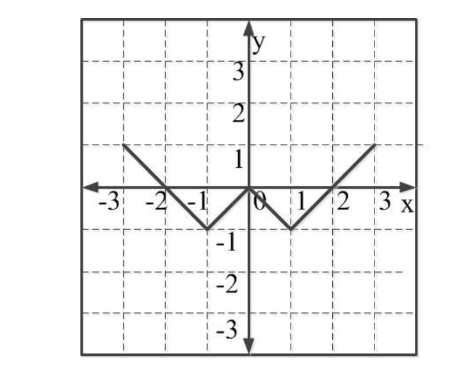
\includegraphics[width = 0.6\columnwidth]{figs/fig3.1.png}
    \caption*{}
    \label{fig:Q9}
\end{figure}
\begin{multicols}{2}
\begin{enumerate}
    \item $y = ||x|+1|-2$ 
    \item $y = ||x|-1|-1$
    \item $y = ||x|+1|-1|$
    \item $y = ||x-1|-1|$
\end{enumerate}
\end{multicols}
 \hfill{(GATE ME 2018)}

\item Consider the following three statements:\\$\brak{i}$ Some roses are red.\\$\brak{ii}$ All red flowers fade quickly.\\$\brak{iii}$ Some roses fade quickly.\\Which of the following statement can be logically inferred from the above statements?
\begin{enumerate}
    \item If $\brak{i}$ is true and $\brak{ii}$ is false, then $\brak{iii}$is false.
    \item If $\brak{i}$ is true and $\brak{ii}$ is false, then $\brak{iii}$ is true.
    \item If $\brak{i}$ and $\brak{ii}$ are true, then $\brak{iii}$ is true.
    \item If $\brak{i}$ and $\brak{ii}$ are false, then $\brak{iii}$ is false.
\end{enumerate}
  \hfill{(GATE ME 2018)}
\begin{center}
\Large
\textbf{END OF THE QUESTION PAPER}
\end{center}
\end{enumerate}
\newpage
\textbf{Q. 1 - Q.55  carry one mark each.}

\begin{enumerate}
\item Four red balls, four green balls and four blue balls are put in a box. Three balls are pulled out of the box at random one after another without replacement. The probability that all the three balls are red is
  \hfill{(GATE ME 2018)}
  
\begin{multicols}{4}
  \begin{enumerate}
    \item $\frac{1}{72}$
    \item $\frac{1}{55}$
    \item $\frac{1}{36}$
    \item $\frac{1}{27}$
\end{enumerate}
\end{multicols}
 
\item The rank of matrix 
 \begin{align}
\begin{bmatrix}
-4 & 1 & -1 \\
-1 & -1 & -1 \\
7 & -3 & 1
\end{bmatrix}
\end{align}

  \hfill{(GATE ME 2018)}
  
\begin{multicols}{4}
\begin{enumerate}
      \item 1
     \item 2
     \item 3
     \item 4
    \end{enumerate}
\end{multicols}

\item According to the Mean Value Theorem, for a continuous function f(x) in the interval $\brak{a,b}$ ,there exists a value $\xi$ in this interval such that $\int_{a}^{b} f(x)\,dx$ =

  \hfill{(GATE ME 2018)}
  
\begin{multicols}{2}
\begin{enumerate}
    \item  $ \ f(\xi)(b - a) $
    \item $\ f(b)(\xi - a)$\\ 
    \item $\ f(a)(b - \xi)$ \quad 
    \item $\ 0 $
\end{enumerate}   
\end{multicols}

\item 
     \( F(z) \) be a function of the complex variable \( z = x + iy \) given by:
    \[
    F(z) = iz + k\, \text{Re}(z) + i\, \text{Im}(z)
    \]
    
    For what value of \( k \) will \( F(z) \) satisfy the Cauchy-Riemann equations?

  \hfill{(GATE ME 2018)}
  
    \begin{multicols}{2}
    \begin{enumerate}
        \item 0
        \item 1
        \item -1
        \item  y 
    \end{enumerate}
    \end{multicols}

    \item 
    A bar of uniform cross-section and weighing 100 N is held horizontally using two massless and inextensible strings S1 and S2 as shown below:

  
  
     \begin{figure}[H]
    \centering
    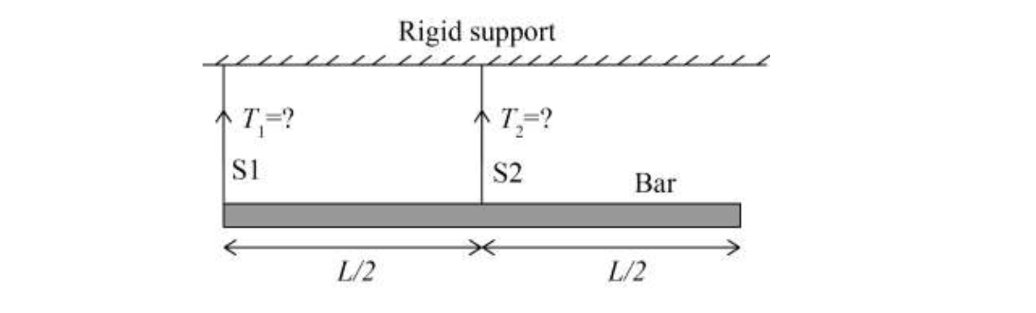
\includegraphics[width = 0.6\columnwidth]{figs/fig3.2.png}
    \caption*{}
    \label{fig:Q3}
    \end{figure}
     The tensions in the strings are
     \hfill{(GATE ME 2018)}
    \begin{enumerate}
 
      
     \item T1=100 N and T2=0N
    \item T1=75 N and T2=25N
        \item T1=0 N and T2=100N
        \item T1=25 N and T2=75N
    \end{enumerate}
\item If $\sigma_1$ and $\sigma_3$ are the algebraically largest and smallest principal stresses respectively, the value of the maximum shear stress is 

  \hfill{(GATE ME 2018)}
  
\begin{multicols}{4}
    \begin{enumerate}
        \item $(\sigma_1+\sigma_3)/2$
        \item $(\sigma_1-\sigma_3)/2$
        \item $\sqrt{(\sigma_1+\sigma_3)/2}$
                \item $\sqrt{(\sigma_1-\sigma_3)/2}$
    \end{enumerate}
\end{multicols}
    \item The equation of motion for a spring-mass system excited by a harmonic force is
 Mx + Kx = F $\cos(\omega t)$
where M is the mass, K is the spring stiffness, F is the force amplitude and $\omega$ is the angular frequency of excitation. Resonance occurs when $\omega$ is equal to
  \hfill{(GATE ME 2018)}
\begin{enumerate}
    
\item $\sqrt{(M/K)}$ 
\item $\frac{1}{2\pi}\sqrt{(M/K)} $
\item $2\pi \sqrt{(M/K)}$
\item  $\sqrt{(K/M)}$ 
\end{enumerate}
\item For an Oldham coupling used between two shafts, which among the following statements
are correct?
I.Torsional load is transferred along shaft axis.
II.A velocity ratio of 1:2 between shafts is obtained without using gears.
III.Bending load is transferred transverse to shaft axis.
IV.Rotation is transferred along shaft axis.

  \hfill{(GATE ME 2018)}
  
\begin{enumerate}
\item  I and III
\item  I and IV
\item  II and III
\item  II and IV
\end{enumerate}

 \item For a two-dimensional incompressible flow field given by
\begin{align*}
\vec{u} = A(x\hat{i} - y\hat{j}), {where } A > 0,
\end{align*}
which one of the following statements is \textbf{FALSE}?

  \hfill{(GATE ME 2018)}
  
\begin{enumerate}
    \item It satisfies continuity equation.
    \item It is unidirectional when \( x \to 0 \) and \( y \to \infty \).
    \item Its streamlines are given by \( x = y \).
    \item It is irrotational.
\end{enumerate}
     \item Which one of the following statements is correct for a superheated vapour?

       \hfill{(GATE ME 2018)}
       
\begin{enumerate}
    \item Its pressure is less than the saturation pressure at a given temperature.
    \item Its temperature is less than the saturation temperature at a given pressure.
    \item Its volume is less than the volume of the saturated vapour at a given temperature.
    \item Its enthalpy is less than the enthalpy of the saturated vapour at a given pressure.
\end{enumerate}
    \item In a linearly hardening plastic material, the true stress beyond initial yielding

  \hfill{(GATE ME 2018)}

\begin{enumerate}
   \item  increases linearly with the true strain
\item  decreases linearly with the true strain
\item  first increases linearly and then decreases linearly with the true strain
\item remains constant
\end{enumerate}

\item The type of weld represented by shaded region in the figure is 
\begin{figure}[H]
    \centering
    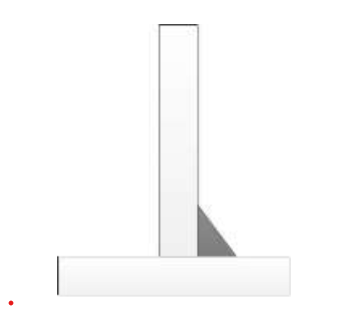
\includegraphics[width = 0.6\columnwidth]{figs/fig3.3.png}
    \caption*{}
    \label{fig:Q17}
    \end{figure}
    \hfill{(GATE ME 2018)}
\begin{enumerate}
    \item groove
    \item spot
    \item fillet
    \item plug
\end{enumerate}

\item Using the Taylor's tool life equation with exponent n = 0.5, if the cutting speed is reduced by 50\%, the ratio of new tool life to original tool life is
\hfill{(GATE ME 2018)}
\begin{multicols}{4}
    \begin{enumerate}
        \item 2
        \item 4
        \item 1
        \item 0.5
    \end{enumerate}
\end{multicols}
 \item A grinding ratio of 200 implies that the
 \hfill{(GATE ME 2018)}
 \begin{enumerate}
\item grinding wheel wears 200 times the volume of the material removed
\item  grinding wheel wears 0.005 times the volume of the material removed
\item  aspect ratio of abrasive particles used in the grinding wheel is 200
\item  ratio of volume of abrasive particle to that of grinding wheel is 200    
 \end{enumerate}
\item Interpolator in a CNC machine
\hfill{(GATE ME 2018)}
\begin{enumerate}
\item controls spindle speed
\item  coordinates axes movements
\item  operates tool changer
\item  commands canned cycle

\end{enumerate}
\item 
The time series forecasting method that gives equal weightage to each of the m most recent observations is
\hfill{(GATE ME 2018)}
\begin{enumerate}
\item Moving average method
\item  Triple Exponential smoothing
\item  Exponential smoothing with linear trend
\item  Kalman Filter
\end{enumerate}

\item The number of atoms per unit cell and the number of slip systems, respectively, for a face-centered cubic $\brak{FCC}$ crystal are
\hfill{(GATE ME 2018)}
\begin{multicols}{4}
    \begin{enumerate}
        \item  3,3
        \item 3,12
        \item 4,12
        \item 4,48
    \end{enumerate}
\end{multicols}
 
\item A six-faced fair dice is rolled five times. The probability (in \%) of obtaining "ONE" at least four times is
\hfill{(GATE ME 2018)}
\begin{multicols}{4}
    \begin{enumerate}
     \item  33.3
\item 3.33

\item  0.33

\item  0.0033
    \end{enumerate}
\end{multicols}
 \item A steel column of rectangular cross-section \( 15\,\text{mm} \times 10\,\text{mm} \) and length \( 1.5\,\text{m} \) is simply supported.
at both ends. Assuming modulus of elasticity, E = 200 GPa for steel, the critical axial load
$\brak{in kN}$ is
(correct to two decimal places).
\hfill{(GATE ME 2018)}

\item A four bar mechanism is made up of links of length 100, 200, 300 and 350 mm. If the 350 mm link is fixed, the number of links that can rotate fully is
\hfill{(GATE ME 2018)}
\item If the wire diameter of a compressive helical spring is increased by 2 \%, the change in spring
stiffness (in \%) is

(correct to two decimal places).
\hfill{(GATE ME 2018)}
\item A flat plate of width L = 1 m is pushed down with a velocity U = 0.01 m/s towards a wall
resulting in the drainage of the fluid between the plate and the wall as shown in the figure.
The average velocity, Uavg of the fluid (in m/s) draining out at the instant shown in the figure is
(correct to three decimal places).
\begin{figure}[H]
    \centering
    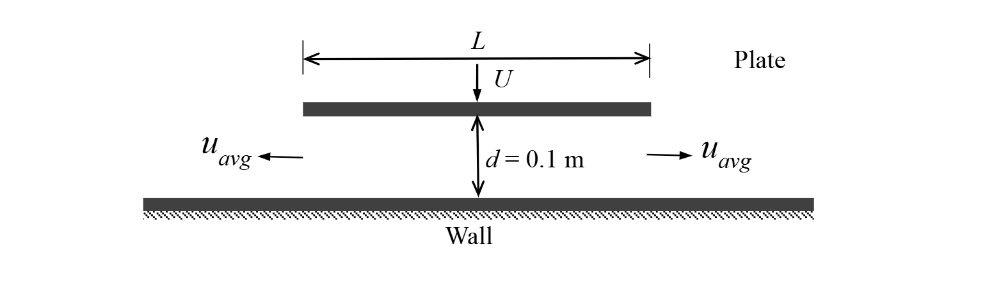
\includegraphics[width = 0.6\columnwidth]{figs/fig3.4.png}
    \caption*{}
    \label{fig:Q22}
    \end{figure}
    \hfill{(GATE ME 2018)}
 .
 \item 
An ideal gas undergoes a process from state 1 (T= 300 K, P1 = 100 kPa) to state 2 $\brak{T_2=600 K, P_2= 500 kPa.}$ The specific heats of the ideal gas are : Cp= 1 kJ/kg-K and Cv=0.7 kJ/kg-K. The change in specific entropy of the ideal gas from state 1 to state 2 $\brak{in kJ/kg-K}$ is

\hfill{(GATE ME 2018)}

\item For a Pelton wheel with a given water jet velocity, the maximum output power from the
Pelton wheel is obtained when the ratio of the bucket speed to the water jet speed
(correct to two decimal places).
piece is

\hfill{(GATE ME 2018)}
\item The height (in mm) for a 125 mm sine bar to measure a taper of 27° 32' on a flat work
(correct to three decimal places).

\hfill{(GATE ME 2018)}

\textbf{Q.26-Q.50 carry 2 marks each}
\item Let X1, X2 be two independent normal random variables with means $\mu_1 \mu_2$ and standard
$\mu_1$ = $\mu_2 =1$  $\sigma_1 =1   \sigma_2 = 2$ 
deviations $\sigma_1   \sigma_2$  respectively. Consider Y =X1-X2;   Then,

\hfill{(GATE ME 2018)}
\begin{enumerate}
\item  Y is normally distributed with mean 0 and variance 1
\item  Y is normally distributed with mean 0 and variance 5
\item Y has mean 0 and variance 5, but is NOT normally distributed
\item  Y has mean 0 and variance 1, but is NOT normally distributed
\end{enumerate}

\item The value of the integral
 
     
    $\iint_{S} \vec{r} \cdot \vec{n} \, dS$
 
over the closed surface S bounding a volume V, where 
\begin{align}
\hat{\mathbf{r}} &= x \hat{i} + y \hat{j} + z \hat{k}
\end{align}
  is the position vector
and n is the normal to the surface S, is
\hfill{(GATE ME 2018)}
\begin{enumerate}
\item V
\item 2V
\item 3V
\item 4V
\end{enumerate}



\item A point mass is shot vertically up from ground level with a velocity of 4 m/s at time, t=0.
It loses 20 \% of its impact velocity after each collision with the ground. Assuming that the
acceleration due to gravity is 10 $m/s^2$ and that air resistance is negligible, the mass stops
bouncing and comes to complete rest on the ground after a total time $\brak{in seconds}$ of
\hfill{(GATE ME 2018)}
\begin{enumerate}
    \item 1
    \item 2
    \item 4
\item $\infty$
\end{enumerate}

\item The state of stress at a point, for a body in plane stress, is shown in the figure below. If the
minimum principal stress is 10 kPa, then the normal stress $\sigma_y$ $\brak{in KPa}$ is
\hfill{(GATE ME 2018)}
\begin{figure}[H]
    \centering
    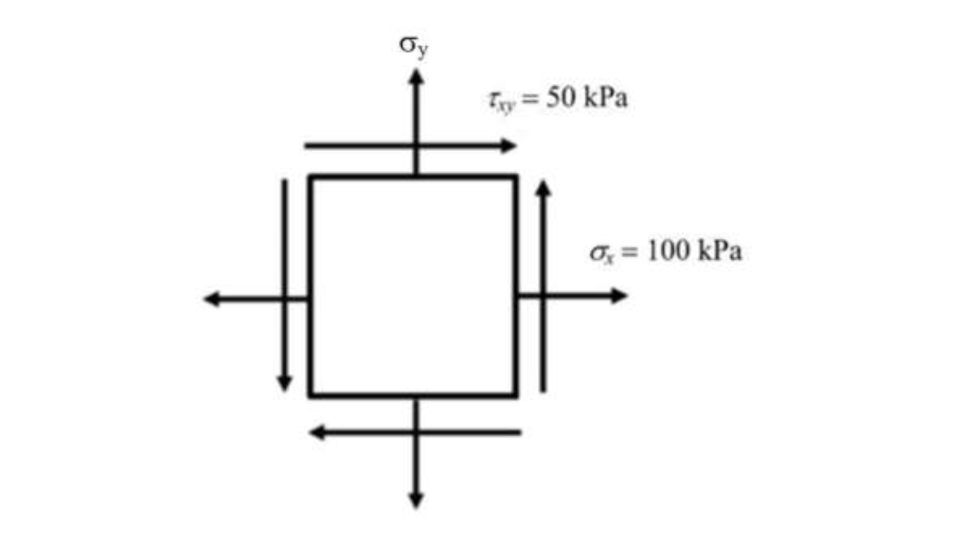
\includegraphics[width = 0.6\columnwidth]{figs/fig3.5.png}
    \caption*{}
    \label{fig:Q28}
    \end{figure}
    \hfill{(GATE ME 2018)}
    \begin{enumerate}
    \item 9.45
    \item 18.88
    \item 37.78
    \item 75.50
    \end{enumerate}
    \item An epicyclic gear train is shown in the figure below. The number of teeth on the gears A, B
and D are 20, 30 and 20, respectively. Gear C has 80 teeth on the inner surface and 100 teeth
on the outer surface. If the carrier arm AB is fixed and the sun gear A rotates at 300 rpm in
the clockwise direction, then the rpm of D in the clockwise direction is
\begin{figure}[H]
    \centering
    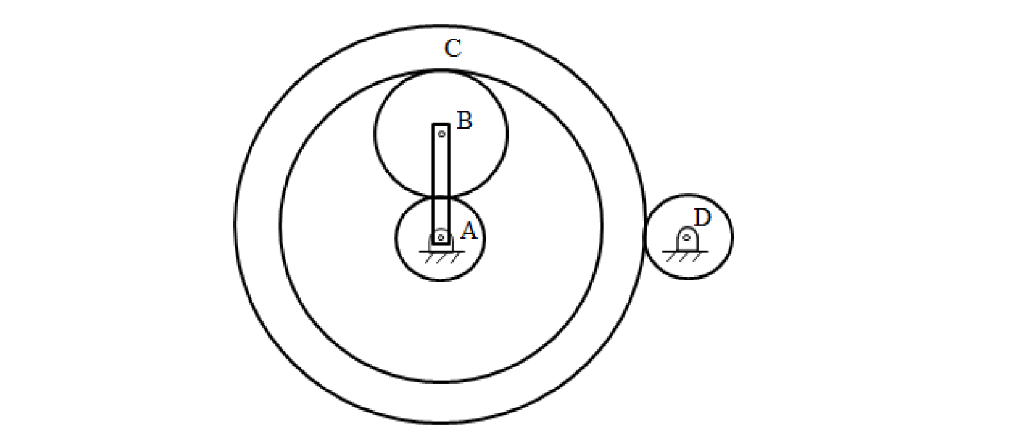
\includegraphics[width = 0.6\columnwidth]{figs/fig3.6.png}
    \caption*{}
    \label{fig:Q29}
    \end{figure}
    \hfill{(GATE ME 2018)}
    \begin{enumerate}
    \item 240
    \item -240
    \item 375
    \item -375
    \end{enumerate}

    \item A carpenter glues a pair of cylindrical wooden logs by bonding their end faces at an angle
of $\theta=30\degree$ as shown in the figure.
\begin{figure}[H]
    \centering
    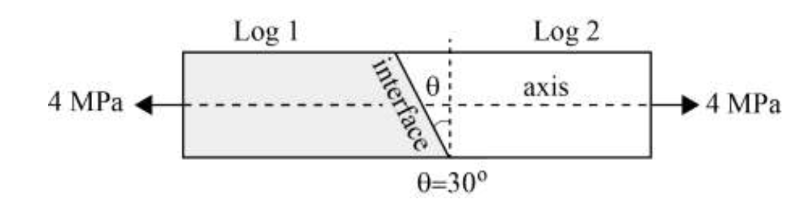
\includegraphics[width = 0.6\columnwidth]{figs/fig3.7.png}
    \caption*{}
    \label{fig:Q31}
    \end{figure}
The glue used at the interface fails if
Criterion 1: the maximum normal stress exceeds 2.5 MPa.
Criterion 2: the maximum shear stress exceeds 1.5 MPa.
Assume that the interface fails before the logs fail. When a uniform tensile stress of 4 MPa is applied, the interface
\hfill{(GATE ME 2018)}
\begin{enumerate}
    \item  fails only because of criterion 1
\item fails only because of criterion 2
\item  fails because of both criteria 1 and 2
\item  does not fail
\end{enumerate}

 \item A self-aligning ball bearing has a basic dynamic load rating $\brak{C10, for 106 revolutions}$ of
35 kN. If the equivalent radial load on the bearing is 45 kN, the expected life $\brak{in 106
revolutions}$ is
\hfill{(GATE ME 2018)}
\begin{enumerate}
    \item below 0.5
\item  0.5 to 0.8
\item  0.8 to 1.0
\item  above 1.0
\end{enumerate}
 \item A tank open at the top with a water level of 1 m, as shown in the figure, has a hole at a height
of 0.5 m. A free jet leaves horizontally from the smooth hole. The distance X $\brak{im\;m}$ where
the jet strikes the floor is
\begin{figure}[H]
    \centering
    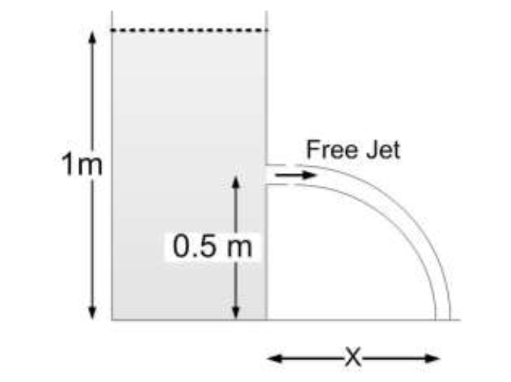
\includegraphics[width = 0.6\columnwidth]{figs/fig3.8.png}
    \caption*{}
    \label{fig:Q33}
    \end{figure}
    \hfill{(GATE ME 2018)}
    \begin{enumerate}
        \item 0.5
        \item 1
        \item 2
        \item 4
    \end{enumerate}
    \item In a Lagrangian system, the position of a fluid particle in a flow is described as 
$x = x_0 e^{-kt}$ and $y = y_0 e^{kt}$ where $t$ is the time while $x_0$, $y_0$, and $k$ are constants. 
The flow is
\hfill{(GATE ME 2018)}
\begin{multicols}{2}
\begin{enumerate}
 \item unsteady and one-dimensional
  \item steady and two-dimensional
  \item steady and one-dimensional
  \item unsteady and two-dimensional
\end{enumerate}
\end{multicols}

\item The maximum reduction in cross-sectional area per pass ($R$) of a cold wire drawing process is
\begin{align*}
R = 1 - e^{-(n+1)},
\end{align*}
where $n$ represents the strain hardening coefficient. For the case of a perfectly plastic material, $R$ is
\hfill{(GATE ME 2018)}
\begin{multicols}{2}
\begin{enumerate}
    
  \item 0.865
  \item 0.826
  \item 0.777
  \item 0.632
\end{enumerate}
\end{multicols}

\item The percentage scrap in a sheet metal blanking operation of a continuous strip of sheet metal
(correct to two decimal places).
as shown in the figure is
\begin{figure}[H]
    \centering
    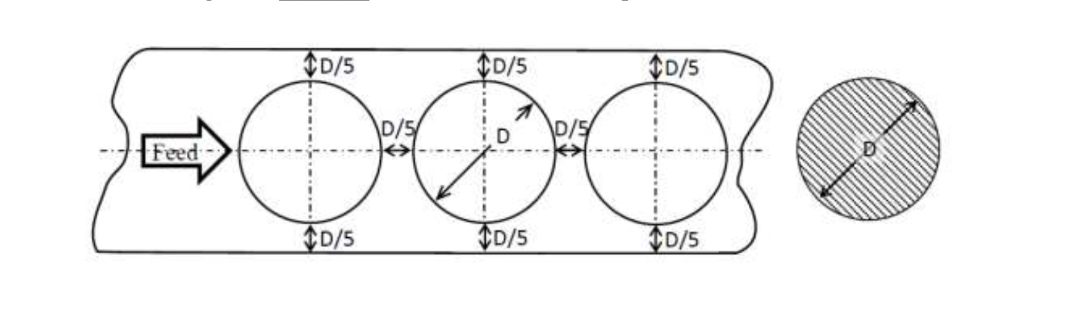
\includegraphics[width = 0.6\columnwidth]{figs/fig3.9.png}
    \caption*{}
    \label{fig:Q36}
    \end{figure} 
    \hfill{(GATE ME 2018)}

  \item An explicit forward Euler method is used to numerically integrate the differential equation 
  \begin{align*}
  \frac{dy}{dt} = y
  \end{align*}
  using a time step of $0.1$. With the initial condition $y(0) = 1$, the value of $y(1)$ computed by this method is \underline{\hspace{3cm}} (correct to two decimal places).
\hfill{(GATE ME 2018)}
  \item $F(s)$ is the Laplace transform of the function 
  \begin{align*}
  f(t) = 2t^2 e^{-t}
  \end{align*}
  $F(1)$ is \underline{\hspace{3cm}} (correct to two decimal places).
  \item A simply supported beam of width 100 mm, height 200 mm and length 4 m is carrying a
uniformly distributed load of intensity 10 kN/m. The maximum bending stress (in MPa) in the beam is 
(correct to one decimal place).
\begin{figure}[H]
    \centering
    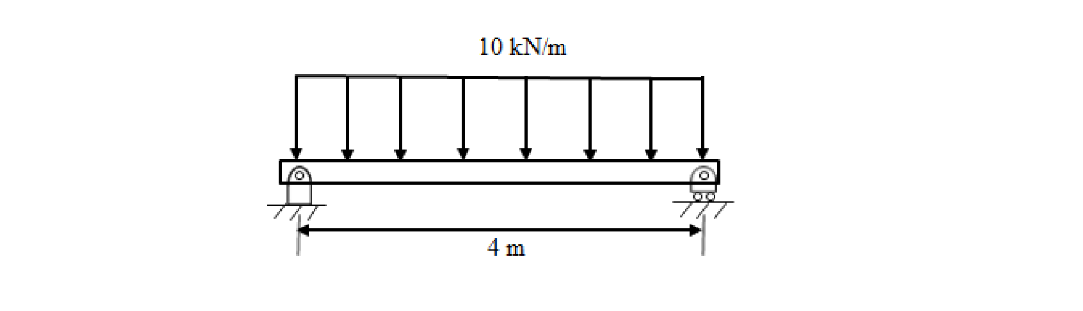
\includegraphics[width = 0.6\columnwidth]{figs/fig3.10.png}
    \caption*{}
    \label{fig:Q39}
    \end{figure} 
\hfill{(GATE ME 2018)}
    \item A machine of mass m = 200 kg is supported on two mounts, each of stiffness
k = 10 kN/m. The machine is subjected to an external force (in N) F(t) = 50 cos 5t.
Assuming only vertical translatory motion, the magnitude of the dynamic force (in N)
transmitted from each mount to the ground is

(correct to two decimal places).
\begin{figure}[H]
    \centering
    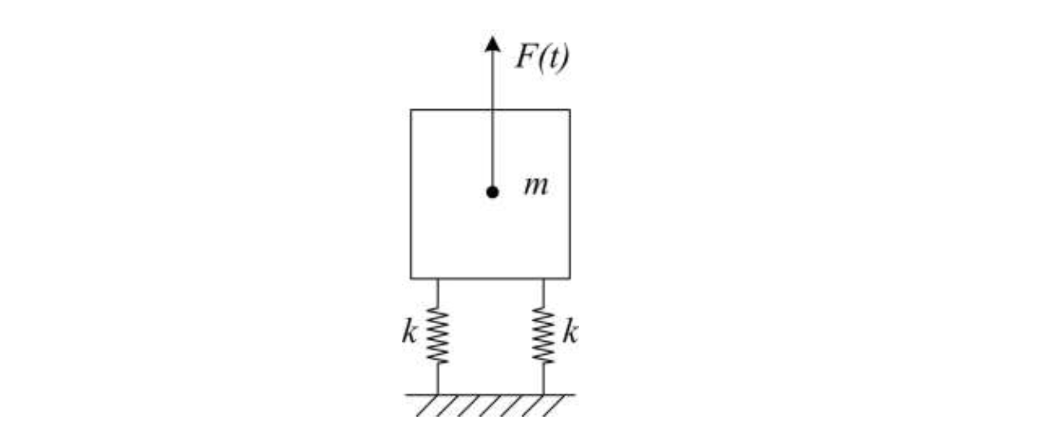
\includegraphics[width = 0.6\columnwidth]{figs/fig3.11.png}
    \caption*{}
    \label{fig:Q40}
    \end{figure} 
    \hfill{(GATE ME 2018)}
    \item A slider crank mechanism is shown in the figure. At some instant, the crank angle is 45° and
a force of 40 N is acting towards the left on the slider. The length of the crank is 30 mm and
the connecting rod is 70 mm. Ignoring the effect of gravity, friction and inertial forces, the
magnitude of the crankshaft torque (in Nm) needed to keep the mechanism in equilibrium is
(correct to two decimal places).
\hfill{(GATE ME 2018)}
\begin{figure}[H]
    \centering
    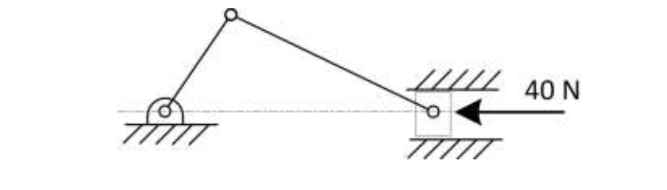
\includegraphics[width = 0.6\columnwidth]{figs/fig3.12.png}
    \caption*{}
    \label{fig:Q41}
    \end{figure} 

    \item A sprinkler shown in the figure rotates about its hinge point in a horizontal plane due to water
flow discharged through its two exit nozzles.
\hfill{(GATE ME 2018)}
\begin{figure}[H]
    \centering
    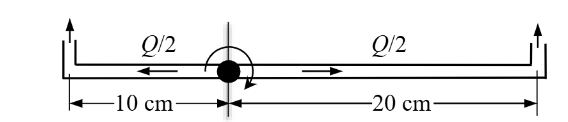
\includegraphics[width = 0.6\columnwidth]{figs/fig3.13.png}
    \caption*{}
    \label{fig:Q42}
    \end{figure} 

The total flow rate Q through the sprinkler is 1 litre/sec and the cross-sectional area of each
exit nozzle is 1 $cm^2$. Assuming equal flow rate through both arms and a frictionless hinge,
the steady state angular speed of rotation $\brak{in rad/s}$ of the sprinkler is
(correct to two decimal places).

\item 
A solid block of 2.0 kg mass slides steadily at a velocity V along a vertical wall as shown in the figure below. A thin oil film of thickness h = 0.15 mm provides lubrication between the block and the wall. The surface area of the face of the block in contact with the oil film is 0.04 m2. The velocity distribution within the oil film gap is linear as shown in the figure. Take dynamic viscosity of oil as 7x$10^-3$ Pa-s and acceleration due to gravity as $10 m/s^2$. Neglect weight of the oil. The terminal velocity V (in m/s) of the block is

 
\hfill{(GATE ME 2018)}

 \centering
 .\begin{figure}[H]
    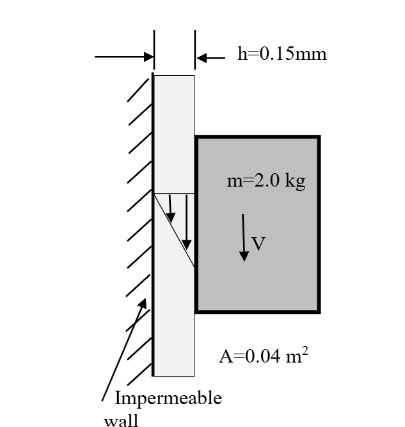
\includegraphics[width = 0.6\columnwidth]{figs/fig3.14.png}
    \caption*{}
    \label{fig:Q43}
    \end{figure} 
\item  A tank of volume $0.05~\text{m}^3$ contains a mixture of saturated water and saturated steam at $200^\circ\text{C}$.  The mass of the liquid present is $8~\text{kg}$. The entropy (in kJ/kg K) of the mixture is \underline{\hspace{3cm}} (correct to two decimal places).  
Property data for saturated steam and water are:
  
  \begin{align*}
  \text{At } 200^\circ\text{C}, \quad & p_{\text{sat}} = 1.5538~\text{MPa} \\
  v_f &= 0.001157~\text{m}^3/\text{kg}, \quad v_g = 0.12736~\text{m}^3/\text{kg} \\
  s_{fg} &= 4.1014~\text{kJ/kg K}, \quad s_f = 2.3309~\text{kJ/kg K}
  \end{align*}
  
  \hfill{(GATE ME 2018)}
  
 \item Steam flows through a nozzle at a mass flow rate of $\dot{m} 0.1~\text{kg/s}$ with a heat loss of $5~\text{kW}$.  The enthalpies at inlet and exit are $2500~\text{kJ/kg}$ and $2350~\text{kJ/kg}$, respectively. Assuming negligible velocity at inlet $C_1 \approx 0$, the velocity $C_2$ steam $\brak{in m/s}$ at the nozzle exit is  (correct to two decimal places).
  \begin{figure}[H]
\centering
    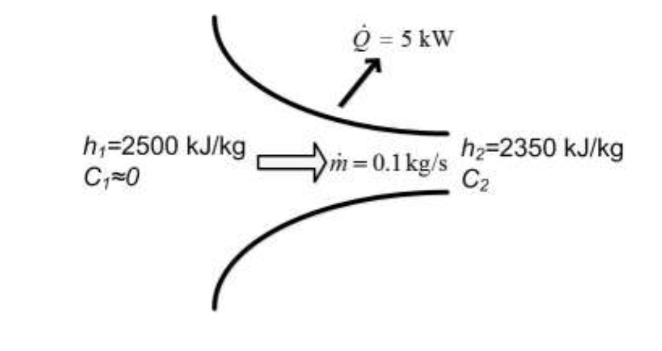
\includegraphics[width = 0.7\columnwidth]{figs/fig3.15.png}
    \caption*{}
    \label{fig:Q45}
    \end{figure}
\item An engine working on air standard Otto cycle is supplied with air at $0.1~\text{MPa}$ and $35^\circ\text{C}$. The compression ratio is $8$. The heat supplied is $500~\text{kJ/kg}$.  
  Property data for air:  
  \[
  c_p = 1.005~\text{kJ/kg K}, \quad c_v = 0.718~\text{kJ/kg K}, \quad R = 0.287~\text{kJ/kg K}
  \]
  The maximum temperature (in K) of the cycle is \underline{\hspace{3cm}} (correct to one decimal place).

\hfill{(GATE ME 2018)}

  \item A plane slab of thickness $L$ and thermal conductivity $k$ is heated with a fluid on one side (P),  
  and the other side (Q) is maintained at a constant temperature, $T_Q$ of $25^\circ\text{C}$, as shown in the figure.  
  \begin{figure}[H]
\centering
    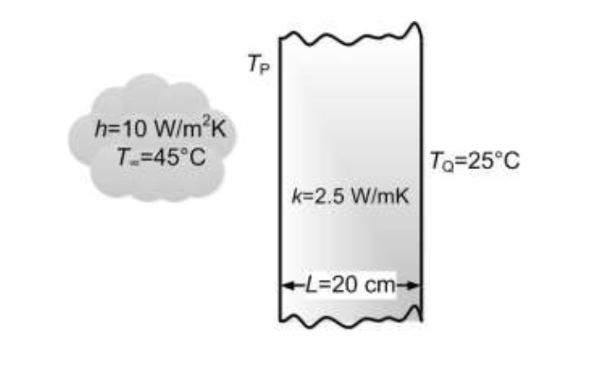
\includegraphics[width = 0.6\columnwidth]{figs/fig3.16.png}
    \caption*{}
    \label{fig:Q47}
    \end{figure}
  
  The fluid is at $45^\circ\text{C}$ and the surface heat transfer coefficient, $h$, is $10~\text{W/m}^2\text{K}$.  
  The steady state temperature, $T_P$ (in $^\circ\text{C}$), of the side which is exposed to the fluid is  
  \underline{\hspace{3cm}} (correct to two decimal places).

  \item The true stress $\sigma$ - true strain $\epsilon$ diagram of a strain hardening material is shown in figure.
First, there is loading up to point A, i.e., up to stress of 500 MPa and strain of 0.5. Then from
point A, there is unloading up to point B, i.e., to stress of 100 MPa. Given that the Young's
modulus E = 200 GPa, the natural strain at point B $(\epsilon_B)$ is
 \hfill{(GATE ME 2018)}
 \begin{figure}[H]
\centering
    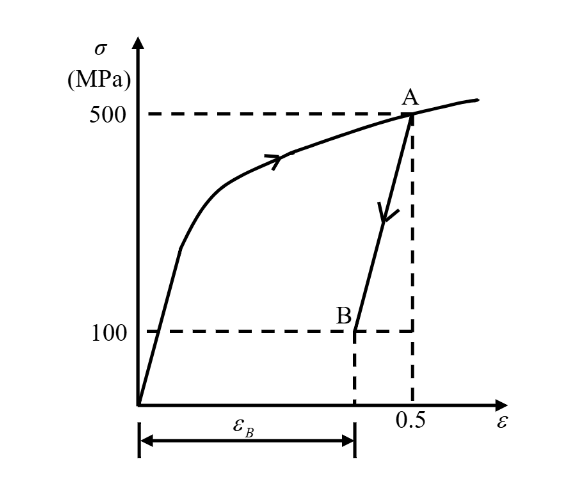
\includegraphics[width = 0.6\columnwidth]{figs/fig3.17.png}
    \caption*{}
    \label{fig:Q48}
    \end{figure}

\item An orthogonal cutting operation is being carried out in which uncut thickness is $0.010~\text{mm}$, cutting speed is $130~\text{m/min}$, rake angle is $15^\circ$ and width of cut is $6~\text{mm}$. It is observed that the chip thickness is $0.015~\text{mm}$, the cutting force is $60~\text{N}$ and the thrust force is $25~\text{N}$. The ratio of friction energy to total energy is $\brak{correct to two decimal places}$

\hfill{(GATE ME 2018)}

\item A bar is compressed to half of its original length. The magnitude of true strain produced in the deformed bar is 
    \hfill{(GATE ME 2018)}
 \item The minimum value of $3x + 5y$ is such that:
    \begin{align*}
        3x + 5y &\le 15 \\
        4x + 9y &\le 8 \\
        13x + 2y &\le 2 \\
        x &\ge 0, \quad y \ge 0
    \end{align*}
     
    \hfill{(GATE ME 2018)}
 \item Processing times (including setup times) and due dates for six jobs waiting to be processed at a work centre are given in the table. The average tardiness (in days) using shortest processing time rule is 
    
\begin{center}
\begin{tabular}{|c|c|c|}
    \hline
    \textbf{Job} & \textbf{Processing time (days)} & \textbf{Due date (days)} \\
    \hline
    A & 3 & 8 \\
    B & 7 & 16 \\
    C & 4 & 4 \\
    D & 9 & 18 \\
    E & 5 & 17 \\
    F & 13 & 19 \\
    \hline
\end{tabular}
\end{center}
\hfill{(GATE ME 2018)}
\item The schematic of an external drum rotating clockwise engaging with a short shoe is shown
in the figure. The shoe is mounted at point Y on a rigid lever XYZ hinged at point X. A force
F = 100 N is applied at the free end of the lever as shown. Given that the coefficient of
friction between the shoe and the drum is 0.3, the braking torque (in Nm ) applied on the drum is 
(correct to two decimal places).
\hfill{(GATE ME 2018)}
\begin{figure}[H]
\centering
    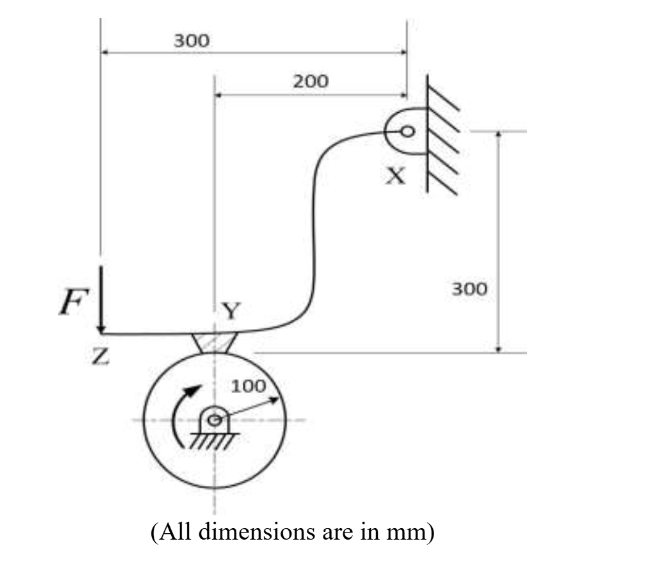
\includegraphics[width = 0.6\columnwidth]{figs/fig3.18.png}
    \caption*{}
    \label{fig:Q53}
    \end{figure}

\item Block P of mass 2 kg slides down the surface and has a speed 20 m/s at the lowest point, Q, where the local radius of curvature is 2 m as shown in the figure. Assuming g = 10 m/s2, the normal force (in N) at Q is
(correct to two decimal places).
\hfill{(GATE ME 2018)}
\begin{figure}[H]
\centering
    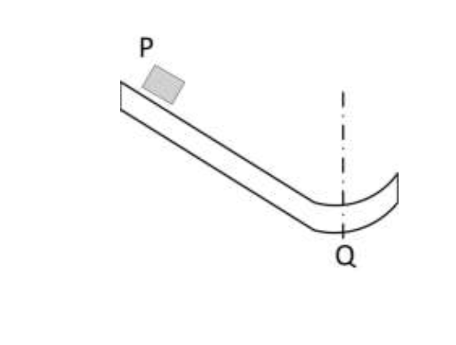
\includegraphics[width = 0.6\columnwidth]{figs/fig3.19.png}
    \caption*{}
    \label{fig:Q54}
    \end{figure}
\item An electrochemical machining (ECM) is to be used to cut a through hole into a 12 mm thick aluminum plate. The hole has a rectangular cross-section, 10 mm x 30 mm. The ECM operation will be accomplished in 2 minutes, with efficiency of 90\%. Assuming specific removal rate for aluminum as 3.44 x $10^(-2) mm^3/(A s)$, the current $\brak{in A}$ required is
(correct to two decimal places).
\hfill{(GATE ME 2018)}
\end{enumerate}
\end{document}


    

 